\subsection{\RU{Запись за пределы массива}\EN{Writing beyond array bounds}}

\RU{Итак, мы прочитали какое-то число из стека явно \IT{нелегально}, а что если мы запишем?}
\EN{OK, we read some values from the stack \IT{illegally}, but what if we could write something to it?}

\RU{Вот что мы пишем:}\EN{Here is what we have got:}

\lstinputlisting{patterns/13_arrays/2_BO/w.c}

\subsubsection{MSVC}

\RU{И вот что имеем на ассемблере:}\EN{And what we get:}

\lstinputlisting[caption=\NonOptimizing MSVC 2008]{patterns/13_arrays/2_BO/w.asm.\LANG}

\RU{Запускаете скомпилированную программу, и она падает. Немудрено. Но давайте теперь узнаем, где именно.}
\EN{The compiled program crashes after running. No wonder. Let's see where exactly does it is crash.}

\clearpage
\myindex{\olly}

\RU{Загружаем в}\EN{Let's load it into} \olly, \RU{трассируем пока запишутся все 30 элементов:}
\EN{and trace until all 30 elements are written:}

\begin{figure}[H]
\centering
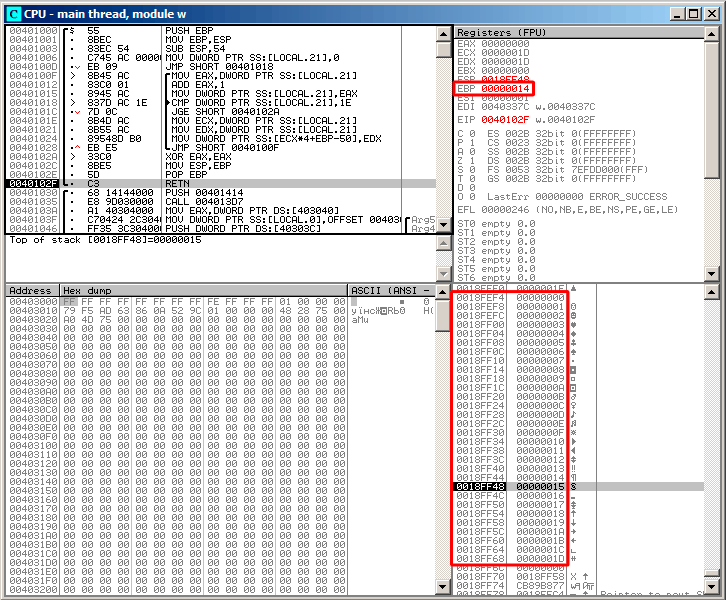
\includegraphics[scale=\FigScale]{patterns/13_arrays/2_BO/olly_w1.png}
\caption{\olly: \RU{после восстановления EBP}\EN{after restoring the value of EBP}}
\label{fig:array_BO_olly_w1}
\end{figure}

\clearpage
\RU{Доходим до конца функции}\EN{Trace until the function end}:

\begin{figure}[H]
\centering
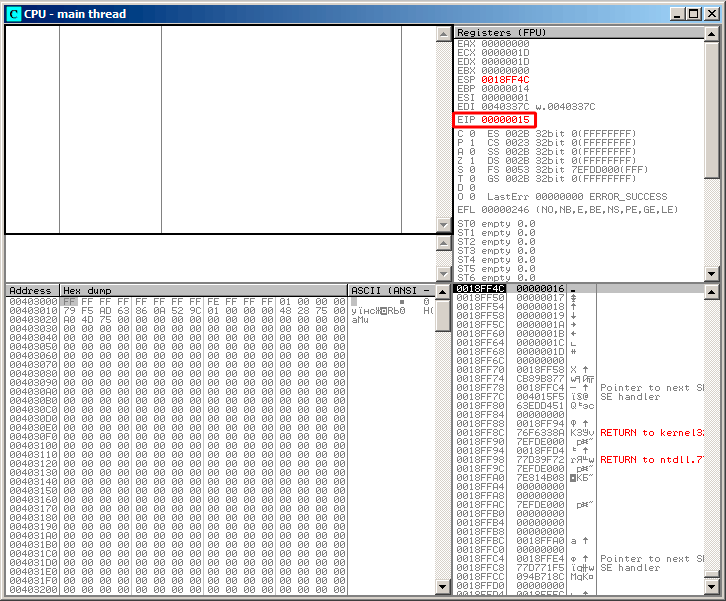
\includegraphics[scale=\FigScale]{patterns/13_arrays/2_BO/olly_w2.png}
\caption{\olly: \RU{EIP восстановлен, но \olly не может дизассемблировать по адресу 0x15}
\EN{EIP was restored, but \olly can't disassemble at 0x15}}
\label{fig:array_BO_olly_w2}
\end{figure}

\RU{Итак, следите внимательно за регистрами.}
\EN{Now please keep your eyes on the registers.}

\RU{\EIP теперь 0x15. Это явно нелегальный адрес для кода~--- по крайней мере, win32-кода! 
Мы там как-то очутились, причем, сами того не хотели. Интересен также тот факт, что в \EBP хранится 0x14, 
а в \ECX и \EDX хранится 0x1D.}
\EN{\EIP is 0x15 now. It is not a legal address for code---at least for win32 code!
We got there somehow against our will.
It is also interesting that the \EBP register contain 0x14,
\ECX and \EDX contain 0x1D.}

\RU{Ещё немного изучим разметку стека.}\EN{Let's study stack layout a bit more.}

\RU{После того как управление передалось в \main, в стек было сохранено значение \EBP. 
Затем для массива и переменной $i$ было выделено 84 байта. Это \TT{(20+1)*sizeof(int)}. 
\ESP сейчас указывает на переменную \TT{\_i} в локальном стеке и при исполнении следующего \INS{PUSH что-либо}, 
\IT{что-либо} появится рядом с \TT{\_i}.}
\EN{After the control flow was passed to \TT{\main}, the value in the \EBP register was saved on the stack.
Then, 84 bytes were allocated for the array and the $i$ variable.
That's \TT{(20+1)*sizeof(int)}.
\ESP now points to the \TT{\_i} variable in the local stack and after the execution of 
the next \TT{PUSH something}, \IT{something} is appearing next to \TT{\_i}.}

\RU{Вот так выглядит разметка стека пока управление находится внутри}
\EN{That's the stack layout while the control is in} \main:

\begin{center}
\begin{tabular}{ | l | l | }
\hline
  \TT{ESP}    & \RU{4 байта выделенных для переменной $i$}\EN{4 bytes allocated for $i$ variable} \\
\hline
  \TT{ESP+4}  & \RU{80 байт выделенных для массива \TT{a[20]}}\EN{80 bytes allocated for \TT{a[20]} array} \\
\hline
  \TT{ESP+84} & \RU{сохраненное значение \EBP}\EN{saved \EBP value} \\
\hline
  \TT{ESP+88} & \RU{адрес возврата}\EN{return address} \\
\hline
\end{tabular}
\end{center}

\RU{Выражение \TT{a[19]=что\_нибудь} записывает последний \Tint в пределах массива (пока что в пределах!)}
\EN{\TT{a[19]=something} statement writes the last \Tint in the bounds of the array (in bounds so far!)}

\RU{Выражение \TT{a[20]=что\_нибудь} записывает \IT{что\_нибудь} на место где сохранено значение \EBP.}
\EN{\TT{a[20]=something} statement writes \IT{something} to the place where the value of \EBP is saved.}

\RU{Обратите внимание на состояние регистров на момент падения процесса. В нашем случае 
в 20-й элемент записалось значение 20. 
И вот всё дело в том, что заканчиваясь, эпилог функции восстанавливал значение \EBP 
(20 в десятичной системе это как раз \TT{0x14} в шестнадцатеричной). 
Далее выполнилась инструкция \RET, которая на самом деле эквивалентна \TT{POP EIP}.}
\EN{Please take a look at the register state at the moment of the crash. In our case,
20 was written in the 20th element. 
At the function end, the function epilogue restores the original \EBP value.
(20 in decimal is \TT{0x14} in hexadecimal).
Then \RET gets executed, which is effectively equivalent to \TT{POP EIP} instruction.}

\RU{Инструкция \RET вытащила из стека адрес возврата (это адрес где-то внутри \ac{CRT}), 
которая вызвала \main), 
а там было записано 21 в десятичной системе, то есть 0x15 в шестнадцатеричной. 
И вот процессор оказался по адресу 0x15, но исполняемого кода там нет, так что случилось исключение.}
\EN{The \RET instruction takes the return address from the stack (that is the address in \ac{CRT}),
which was called \main),
and 21 iss stored there (\TT{0x15} in hexadecimal).
The CPU traps at address \TT{0x15},
but there is no executable code there, so exception gets raised.}

\myindex{\BufferOverflow}
\RU{Добро пожаловать! Это называется}
\EN{Welcome! It is called a} \IT{buffer overflow}\footnote{\href{http://go.yurichev.com/17132}{wikipedia}}.

\RU{Замените массив \Tint на строку (массив \Tchar), нарочно создайте слишком длинную строку, 
передайте её в ту программу, 
в ту функцию, которая не проверяя длину строки скопирует её в слишком короткий буфер, 
и вы сможете указать программе, по какому именно адресу перейти. 
Не всё так просто в реальности, конечно, но началось всё с этого%
\footnote{Классическая статья об этом: \cite{Phrack4914}}.}
\EN{Replace the \Tint array with a string (\Tchar array), create a long string deliberately
and pass it to the program, to the function, which doesn't check the length of the string and copies it in a short buffer,
and you'll able to point the program to an address to which it must jump.
It's not that simple in reality, but that is how it emerged%
\footnote{Classic article about it: \cite{Phrack4914}.}}

\subsubsection{GCC}

\RU{Попробуем то же самое в GCC 4.4.1. У нас выходит такое:}
\EN{Let's try the same code in GCC 4.4.1. We get:}

\lstinputlisting{patterns/13_arrays/2_BO/w_gcc.asm}

\RU{Запуск этого в Linux выдаст:}\EN{Running this in Linux will produce:} \TT{Segmentation fault}.

\myindex{GDB}
\RU{Если запустить полученное в отладчике GDB, получим:}
\EN{If we run this in the GDB debugger, we get this:}

\begin{lstlisting}
(gdb) r
Starting program: /home/dennis/RE/1 

Program received signal SIGSEGV, Segmentation fault.
0x00000016 in ?? ()
(gdb) info registers
eax            0x0	0
ecx            0xd2f96388	-755407992
edx            0x1d	29
ebx            0x26eff4	2551796
esp            0xbffff4b0	0xbffff4b0
ebp            0x15	0x15
esi            0x0	0
edi            0x0	0
eip            0x16	0x16
eflags         0x10202	[ IF RF ]
cs             0x73	115
ss             0x7b	123
ds             0x7b	123
es             0x7b	123
fs             0x0	0
gs             0x33	51
(gdb) 
\end{lstlisting}

\RU{Значения регистров немного другие, чем в примере win32, потому что разметка стека чуть другая.}
\EN{The register values are slightly different than in win32 example, 
since the stack layout is slightly different too.}
